\chapter{Usage Guide}
\label{chap:usage_guide}
HighwayToSafety is a software designed for a lot of different users with a lot
of different interfaces. However, every user just needs to know how the
interface, that he is going to work with, functions. The coordinators of the
firemen and policemen for instance have to work with a very simple application.
It's easy to use because they eventually work with it on the site of the
accident, where it might be very noisy and chaotic.
The administrators and emergency central work with a little more complex
application, which allows them to manage and organise ressources such as human
ressources, equipment and vehicles.

This section is aimed at describing the general use of each actor by using
procedure descriptions. The description of the processes is organised in a way
to facilitate learning by presenting simpler, more common, or initial processes 
before more complex, less utilised, or subsequent processes.

\textbf{(including installation procedures)}.

 \cite{armour01usecase} \textbf{BUT its content must be as low level as possible with actual values}:
\vspace{0.5cm}
\hrule
\begin{lyxlist}{UC1}
\small{
\item [\textbf{Use~Case:}] ProcessMissionOne
\item [\textbf{Scope:}] Crisis Management System (\emph{CMS})
\item [\textbf{Primary Actor}:] Coordinator John
\item [\textbf{Secondary Actor}:] FirstAidWorker Bob,\\
                  ExternalResourceSystem (ERS)
\item [\textbf{Intention:}]The intention of the Coordinator is to process mission with ID equal to 1.
\item [\textbf{Level}:]Sub-functional level
\item [\textbf{Main~Success~Scenario}]:\\
1. \emph{John} instructs the \emph{CMS} to process a specific mission.\\
2. \emph{CMS} selects the internal worker \emph{Bob} to execute the mission.\\
3. \emph{CMS} instructs `\emph{Bob} to behave as \emph{FAW}.\\
4. \emph{Bob} informs to the \emph{CMS} of his arrival.\\
5. \emph{Bob} executes the mission.\\
6. \emph{Bob} informs to the \emph{CMS} the mission outcome.


\item [\textbf{Extensions}]:\\
2.a None internal worker can execute the mission.\\
\hspace*{0.5cm} 2.a.1 \emph{CMS} requests an external resource to \emph{ERS}.\\
\hspace*{0.5cm} 2.a.2 \emph{ERS} informs \emph{CMS} that the request can be processed.\\
\hspace*{1.4cm} Use case continues at step 3.

}

\end{lyxlist}
\hrule
\vspace{0.5cm}

\Remark{Graphical User Interfaces (GUIs)}: include GUIs screenshots to show the
different stages of the process while its is performed by the actor.



\section{Actors common procedures}
Common procedures to several actors are grouped in this section to avoid
redundancy.

\subsection{suGlobalManagementOfEvent}

\begin{lyxlist}{UC1}
\small{
\item [\textbf{Use~Case:}] suGlobalManagementOfEvent
\item [\textbf{Scope:}] Enterprise level
\item [\textbf{Primary Actor}:] Walter: Human Witness,\\ 
						        Camille: Central Coordinator,\\
								Fabio: Firemen Coordinator,\\
								Ted: Tow-truck driver,\\ 
								Polo: Police Coordinator
\item [\textbf{Secondary Actor}:] Orange: Communication Company
\item [\textbf{Intention:}] The intention of this procedure is to have a new
event\\ registered into the system and have all the required resources\\ arrive
at the accident’s location.
\item [\textbf{Level}:] Summary level
\item [\textbf{Main~Success~Scenario}]:
\begin{enumerate}
  \item Walter contacts by phone Camille at the Emergency Central.
  \item Camille sends a message to HTS(i.e. Highway to Safety) to request
  coordinates of Walter's phone number 00352 691 12 34 56.
  \item HTS sends a message to Orange to receive the coordinates of the user
  with phone number 00352 691 12 34 56.
  \item Orange sends coordinates of phone number 00352 661 123 123 to HTS.
  \item HTS sends Walter's coordinates to Camille.
  \item Camille asks the system to create a new event associated to the crisis
  with the following information:
  \begin{enumerate}
  \item Walter (name)
  \item Witness (actor type)
  \item ``Highway carcrash with two cars involved'' (comment)
  \end{enumerate}
  \item HTS creates the new event with the information given by Camille and
  generates a new crisisID:1 to the event.
  \item HTS adds phone number and coordinates of phone number to the event 1.
  \item HTS sends a request to dispatch a team to the nearest, available Firemen
  Coordinator Fabio.
  \item HTS sends a request to dispatch a tow-truck to the nearest, available
  Tow-truck driver Ted.
  \item Fabio sends a message to HTS that his team is on its way to the
  accident’s location.
  \item Ted sends a message to HTS to refresh the map.
  \item Ted sends a message to HTS (``I will arrive in 30 minutes'').
  \item Ted sends a message to HTS that he is on his way to the accident’s
  location.
  \item Fabio sends a message to HTS that his team has arrived at the accident’s
  location.
  \item Fabio sends a message to HTS that they require a Police Team.
  \item HTS sends a request to dispatch a team to the Police Coordinator Polo.
  \item Polo sends to HTS that his team is on its way to the accidents
  location.
  \item Ted sends a message to HTS that he has arrived at the accident’s
  location.
  \item Polo sends a message to HTS that his team has arrived at the accident’s
  location.
\end{enumerate}
}
\end{lyxlist}



\begin{minipage}{0.72\textwidth}
\begin{figure}[H]
\caption{New Event window}
\includegraphics[width=1.0\textwidth]{GetLocation.eps}
\end{figure}
\end{minipage} \hfill
\begin{minipage}{0.23\textwidth}
\begin{itemize}
\item 1.By pressing the ``Get Location'' button Camille asks the system to
get the location of the phone number of the witness.
\item 2. These fields are filled by Camille with the corresponding
information as described in step 6 of the main success scenario.
\end{itemize}
\end{minipage}

\begin{minipage}{0.72\textwidth}
\begin{figure}[H]
\caption{Change Status GUI}
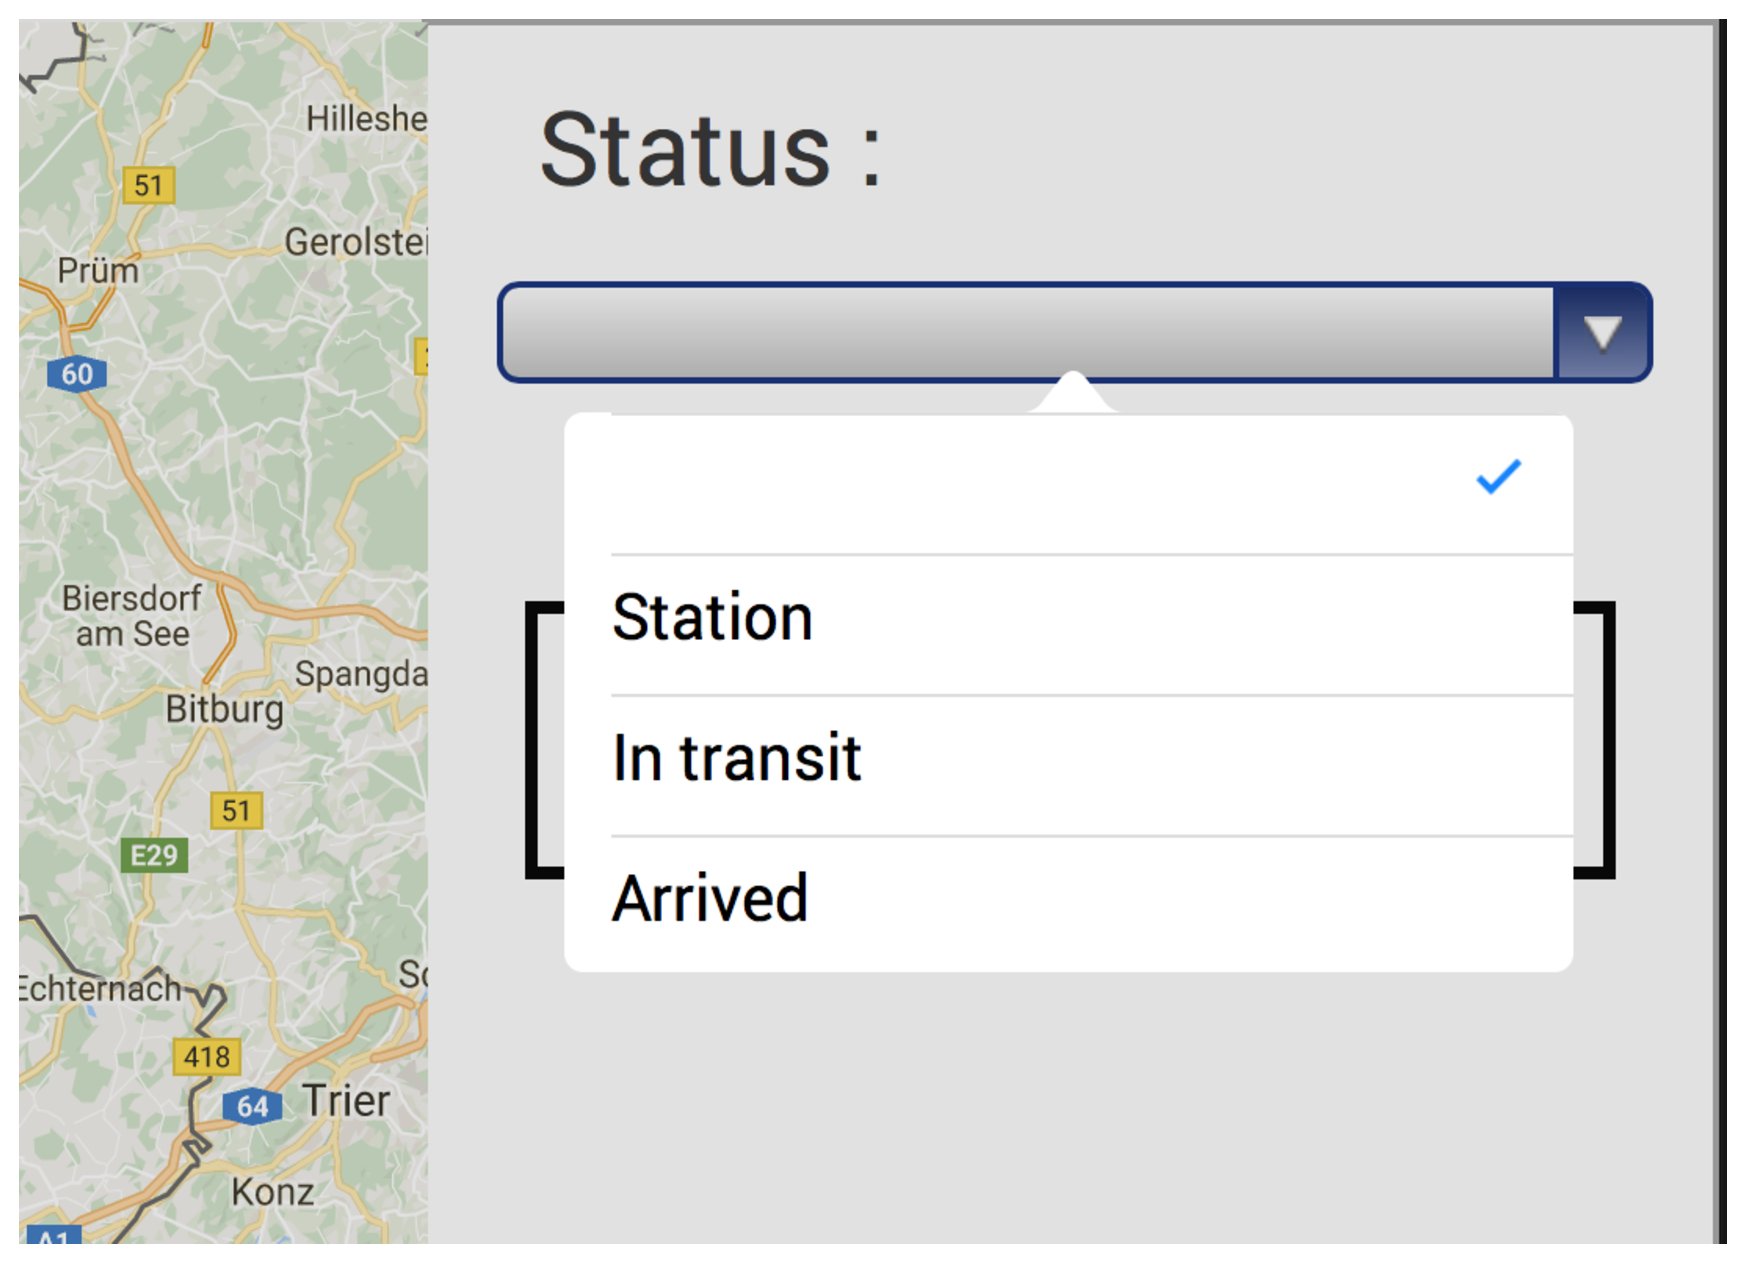
\includegraphics[width=1.0\textwidth]{Ipad_status.eps}
\end{figure}
\end{minipage} \hfill
\begin{minipage}{0.23\textwidth}
\begin{itemize}
\item As described in steps 11, 14, 15, 18, 19, 20 of the main success scenario,
the coordinators can update their status to ``Station'', ``In
transit'' or to ``Arrived''.
\end{itemize}
\end{minipage}



\begin{minipage}{0.72\textwidth}
\begin{figure}[H]
\caption{Ipad chat window}
\includegraphics[width=1.0\textwidth]{Ipad_Messages.eps}
\end{figure}
\end{minipage} \hfill
\begin{minipage}{0.23\textwidth}
\begin{itemize}
\item 1. Ted writes a message to the emergency central by using the textfield.
\item 2. Fabio uses the pre-programmed makros to call for police assistance.
\item 3. With the plus and minus buttons Fabio can specify how much
assistance he needs.
\end{itemize}
\end{minipage}






\subsection{MyCommonProcedure2}


\section{My-Actor1 procedures}

\subsection{MyProcedure1}

\subsection{MyProcedure2}




\section{My-Actor2 procedures}
\subsection{MyProcedure1}
\subsection{MyProcedure2}


\section{My-Actor3 procedures}

\subsection{MyProcedure1}
\subsection{MyProcedure2}















